\glsresetall{} 
\chapter{Software Architecture}


\section{POPS Architecture}

The \gls{pops} is made up of several distinct components separated into
services.  Each service has its own Docker5 container. Containers are similar
to virtual machines in that they simulate an operating system but, unlike
virtual machines, they do not simulate the underlying hardware. This makes
containers much more lightweight, while also retaining the benefits of having a
standardized environment where dependencies are packaged with their source
code. Containers make deploying and maintaining \gls{pops} much easier since
installation does not require managing dependencies and tweaking environment
variables. In this way, a \gls{pops} user does not need to be as familiar with
the software as a developer to run it. Each service is its own Python web
server.  In this way, they may be interacted with via a RESTful API. That
being, HTTP requests can be made to retrieve information or perform
calculations. Each service also provides its own automatically generated
documentation that can be accessed through a web browser. This documentation
outlines possible API calls as well as their input and output data formats.
This allows a user to quickly see the capabilities of a service without
accessing the source code. Currently, \gls{pops} has 4 main services; they are
the: Mission Model, Propagator, Database, and Access Time Utilities,  Mission
Model.

\section{General Service Architecture}

Every service contains the same basic components so it is worth discussing
services generally and then going into specifics in subsequent sections. These
components are: the dockerfile, a main Python script, a models file, service
specific scripts.

To review, a docker container is a virtual environment, which is a simulated
operating system. A container can be created from an image and an image canbe
built from a Dockerfile. As such, the Dockerfile is the fundamental text
document that is used to assemble an image. It specifies: the operating system
that should be used, what files should be included in the container, and what
commands should be run upon container creation. By specifying an operating
system, we can tailor a service to any environment that best suits the service's
needs. They can use windows, the latest version of Ubuntu, or a lightweight
tailored linux distrubution that only contains the tools a service needs. In
this way, one service can be running Ubuntu 20.04 for ease of development, and
another service can be running Windows 10. In this way, \gls{pops} is not
limited by the operating system it is developed in. Files may  be added to a
container simply by pointing to their location in the host's file system upon
image creation. Finally, when a container is first created from an image, a
conatiner will need to install all of the necessary dependencies. In general,
this will either be Ubuntu packages, a version of Python, and Python libraries.
In this way, dependencies can easily be tracked. The last command that is
executed is the command that starts a service's main script.

Theoretically, all of the code for a service could live in the main Python file
but, if this were the case, it would quickly balloon and become unwieldy to work
with so functionality is split into multiple scripts. The main script serves a
number of functions. Its purpose is to handle all of the web-server aspects of
the service. Functions such as: creating the web-server, setting server
parameters, setting up environment variables, and handling API calls. Setting up
the webserver is fairly straightforward since open source libraries are used to
handle all of the low-level functionality and implementation. What is most
important is specifying potential HTTP requests. These requests are how a
service may be interacted with by a user, their browser, or by other services.
The parts that must be specified are the: 

\begin{itemize}
    \item Request type (GET, POST, PUT, etc.), 
    \item Path to the request, 
    \item Response type (JSON, Plain Text, HTML, etc.), 
    \item Input variables if applicable, and the 
    \item Function that is called when a request is received.
\end{itemize}

For GET requests, the input variables are generally straightforward since the
only input variables that can be used must be explicitly stated in the request
itself. But, for POST requests or other requests that contain information in
the body of the request, the format of the input data must be defined or else
the web server will fail the request as being unprocessable. These input
definitions are stored in the models file. Python is a dynamically typed
language so variables do not need to be assigned a type upon creation. To
ensure input data conforms with what is expected by the api, the Python library
\texttt{Pydantic} is used to enforce data types at runtime. These Pydantic
input definitions are contained in the models file. The remainder of the files
in a service are specific to the service itself.

Having multiple Docker containers becomes cumbersome when a user or a developer
wishes to build new images or run new containers from their images. To manage
all of the different services, another tool is used called "Docker Compose".
From a single configuration file, mutliple services may be started, stopped, or
built from their source code. Services may also have their image name,
container name, and port number set through the configuration file. This vastly
simplies configuration for \gls{pops} as a whole. Another benefit of using
Docker Compose is that it also creates a bridget network for the containers
Docker Compose creates. Containers are intended to be standalone units but a
bridge network allows containers to communicate with each other directly.


\section{Propagator Service}

The Propagator service handles ephemeris generation for \gls{pops}.
Ephemerides are a crucial component for every subsequent step along the
planning process so it is essential that they are well formed. Consolidating
ephemeris generation for the entire tool ensures that only one area of the code
needs to be developed and validated.

Currently, the main method of orbital propagation for \gls{pops} is with the
\gls{sgp} model series of algorithms, specifically SGP4/SDP4 referred to as
just ‘SGP4’. SGP4 is an analytical method of approximating orbital state
vectors at corresponding epochs in the \gls{teme} \gls{eci} coordinate frame,
given a NORAD \gls{tle}.  \gls{tle}s are readily provided by the United States
Space Force through Space-Track6 or CelesTrak7. The \gls{teme} coordinate frame
is not particularly useful so part of the Propagator service’s purpose is
transforming the orbit vectors into a coordinate system required by other parts
of \gls{pops}.  Currently, the two possible output reference frames are the
\gls{gcrs}, which is an \gls{eci} reference frame, and the \gls{wgs}, which is
an \gls{ecef} reference frame.  Depending on the application, it is sometimes
useful to use \gls{eci} or \gls{ecef} reference frames, so both are made
available by the service.  Given a \gls{tle}, a time range, a step size, and a
coordinate system, the Propagator service generates an Ephemeris for the
provided time range in a variety of output formats.

There are two scripts that handle all of the functionality for the Propagator
service. The first is the main script which, as discussed previously, takes
requests, organizes the input data, and formats the output data. The actual
propagation and coordinate change logic is stored in the propagation script.
Open source libraries are used to perform the SGP4 and coordinate change
algorithm so the main focus of the script is to ensure the input data conforms
with the expected format.  

\begin{figure}[h]
    \centering
    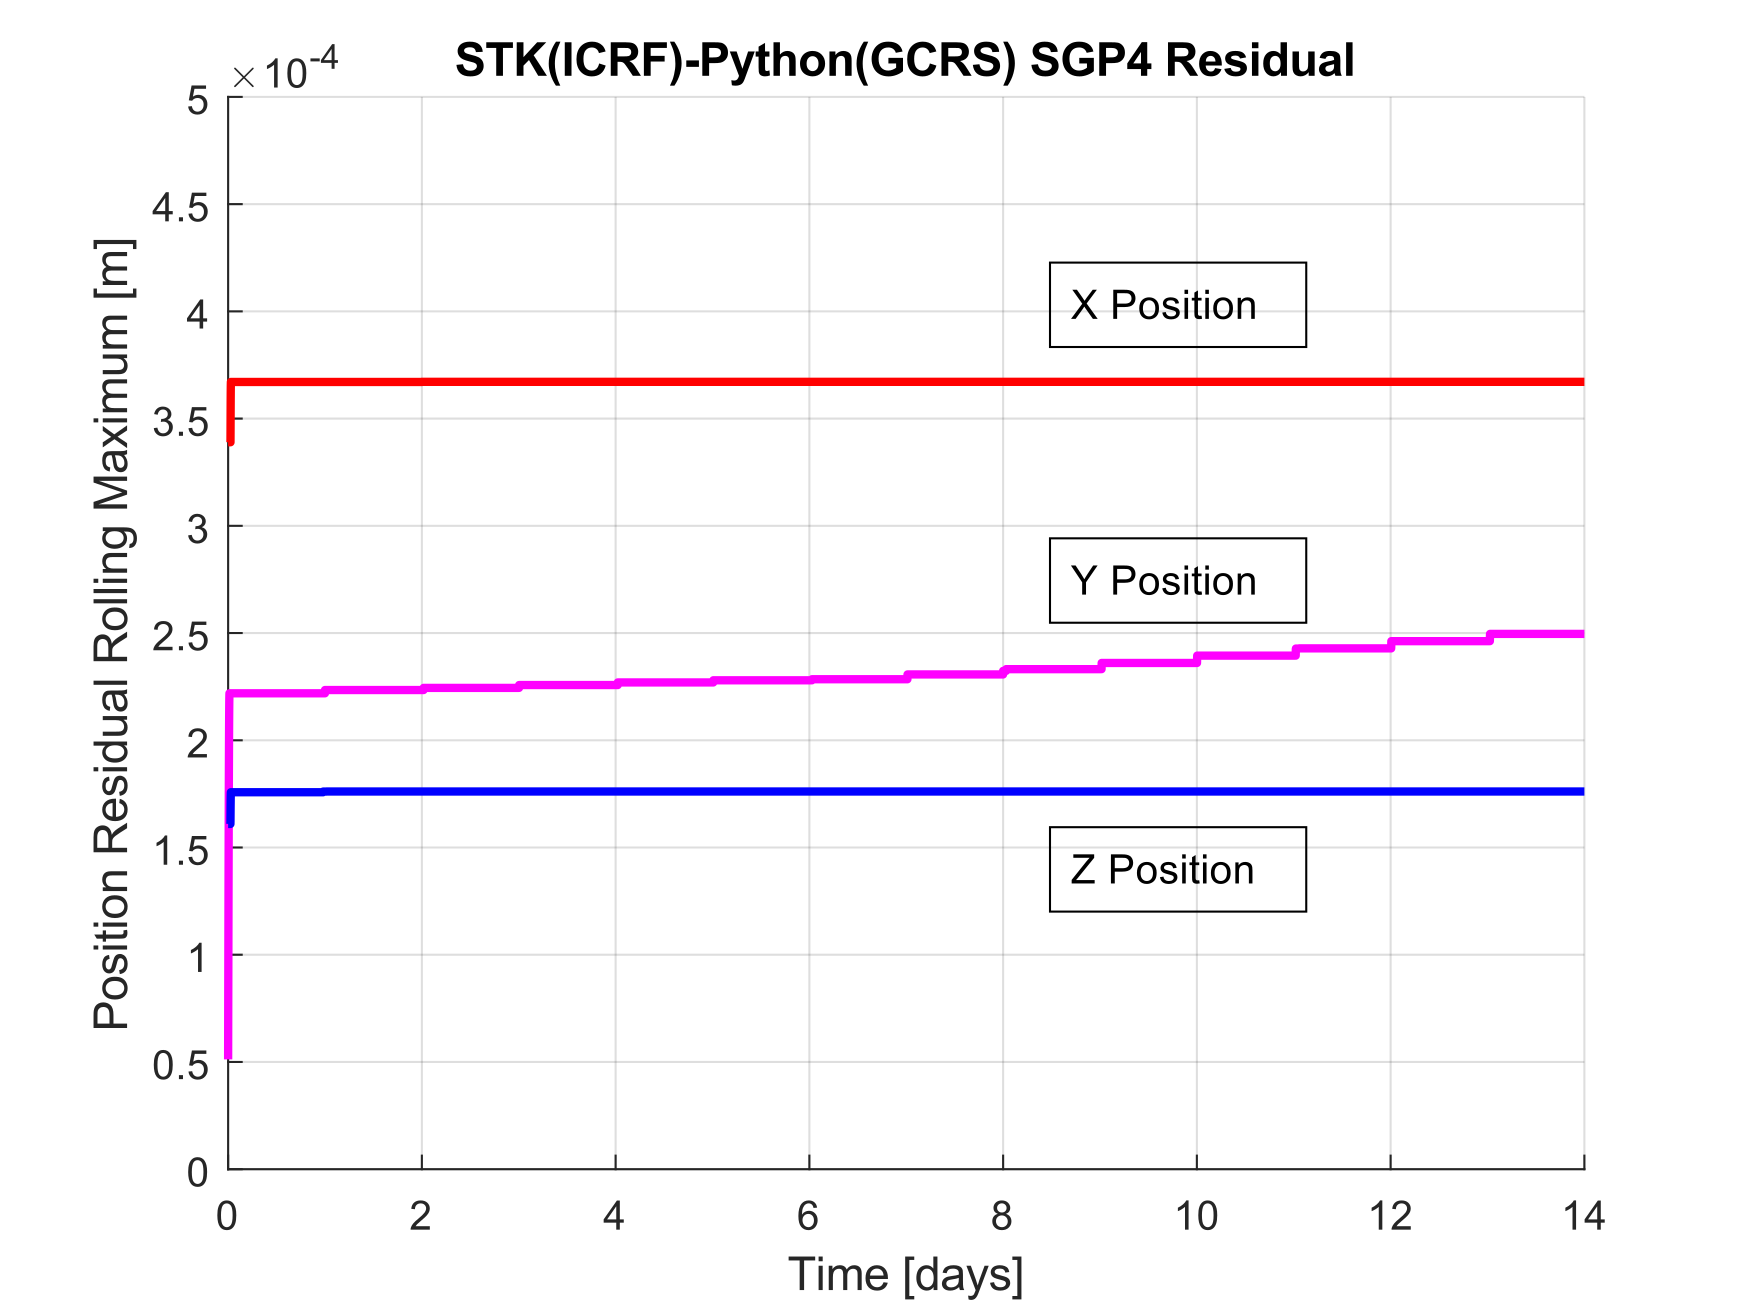
\includegraphics[width=0.7\textwidth]{STK_PY_residual-2.png} 
    \caption{Residual Difference \gls{stk} vs. Python}
    \label{fig:stk_py} 
\end{figure}

It is very easy to generate Ephemeris data. What is difficult is validating it.
The benchmark for validation is \gls{stk} since it has its own SGP4 ephemeris
generation capabilities. If operators did not use POPS, their best alternative
would be to set up scenarios manually in \gls{stk}. As such, using it as ground
truth is valid in this case. Both \gls{stk} and the \gls{pops} implementation
of SGP4 us the same source8: Revisiting Spacetrack Report \#39. As such, they
should provide the same results. One difference to note is that \gls{stk} uses
the \gls{icrf} \gls{eci} coordinate system but the propagator service uses
\gls{gcrf}.  This difference is acceptable since these reference frames are
approximately identical10. The procedure for validating the Propagator service
was first to select a \gls{tle}, a time range, a time step, and a coordinate
system.  Next was to generate Ephemerides from \gls{stk} and the propagation
service.  Finally, the results were compared. One such comparison can be seen
in Figure \ref{fig:stk_py}. Here, the peak position residual was 0.37mm for the position along
the x-axis. The main purpose of this exercise is to ensure that the Python
libraries are being used correctly and that their output data is acceptable.
From this result, it is clear that the methods are identical and the difference
was most likely due to slight implementation differences. 

Another responsibility of the Propagator service is to determine a list of
passes for a given ephemeris. Having an entire ephemeris may be cumbersome for
some calculations so it makes sense to split a whole ephemeris into multiple
components. A `pass' is of course a completely general term so in this context
it is defined as the period between south-to-north hemisphere crossings as this
definition was chosen because it is easy to calculate an equator crossing. This
is where the z-position of a spacecraft goes from negative to positive.
\hl{See algorithm ?? for a discussion on how crossings are found}.

Part of the benefit of having the Propagator as its own service is that if a
more accurate algorithm is desired for orbital propagation, only the Propagator
service needs to be changed and the rest of \gls{pops} can be left as is.


\subsection{Access Time Utilities}

The ATU service provides the basic building blocks for
constraining observation opportunities. These can be added to depending on a
mission’s need. The \gls{atu} service currently supports calculating: ground station
access times, swath generation, horizon swath generation, and polygon
intersection with a swath. These will be discussed in detail in their own
section.  



\section{Mission Model}
 
The Mission Model service is the service that contains the main logic for most
of \gls{pops}'s functionality and front-end \gls{gui}. When a user interacts
with \gls{pops}, they are interacting with the Mission Model service. As such,
it is quite large and has a number of responsibilities. Some of them are:

\begin{outline} 
    \1 Database management,
    \1 Displaying an interactable front-End User Interface,
    \1 Earth Visualization,
    \1 Plan Configuration, and
    \1 Scheduling.
\end{outline}


\begin{figure}[h]
    \centering
    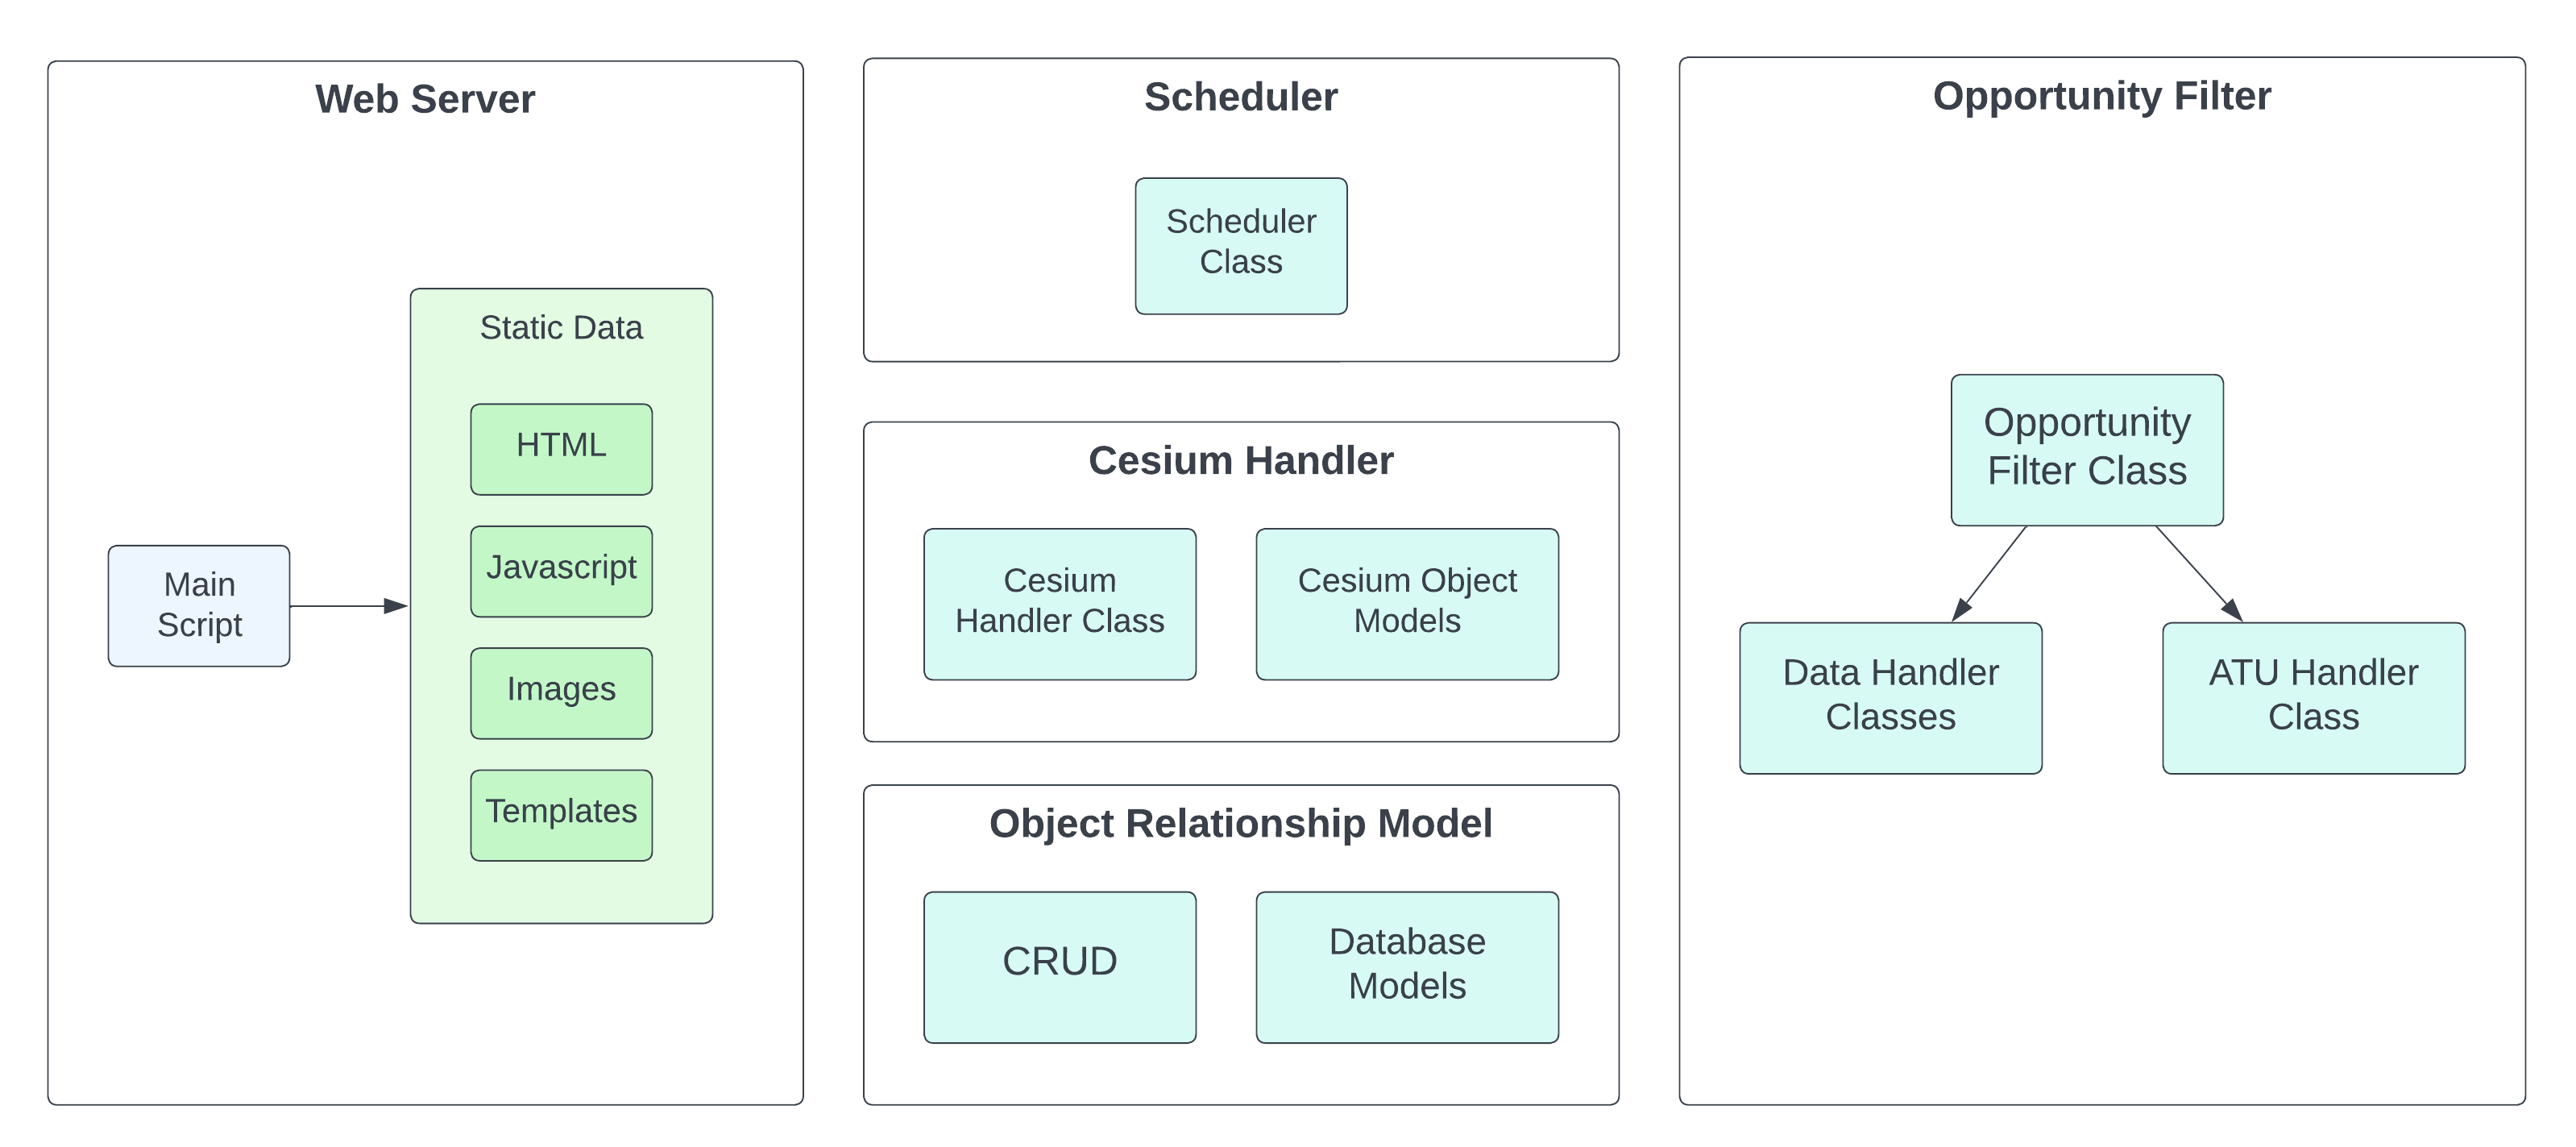
\includegraphics[width=0.7\textwidth]{Mission Model.png} 
    \caption{High Level Structure of Mission Model Service}
    \label{fig:mission_model} 
\end{figure}

A high-level overview of the Mission Model service can be seen in Figure
\ref{fig:mission_model}. There are many components but we will go through them
one by one.

\subsection{Main} 

The main Python script acts as the base for the entire Mission Model service.
Its purpose is to, among other things, set up the web server, load environment
variables, instantiate the handler classes, and associate API calls with their
callback functions. Setting up the web server is the same as with any other
service. The environment variables range from server metadata to addresses of
other containers. There are a number of utility classes that handle various
aspects of \gls{pops}. These are the: scheduler, \gls{atu} handler, data
handler, and opportunity filter classes. They will be discussed in the
following sections. The most important part of the main service is defining API
calls. If a user wishes to interact with \gls{pops}, they must enter a link on
the their browser, that information is then sent to the web server, and a
callback function in the Mission Model service is called. It is the Mission
Models responsibility to consolidate information, whether that be from the
database, through HTML templates, or new information that must be calculated.
The Mission Model service does very few actual calcualtions, its only purpose
is to organize information and call functions as necessary to serve a request.
Currently, the main service is large and difficult to navigate because of its
size. In the future, it will be refactored to a number of sub-scripts that
handle specific functionality in the service.

\subsection{Object Relationship Mapping}

The Database is its own service but the Mission Model is currently the only
service that interacts with it. It does so by using an \gls{orm}. An \gls{orm}
is a method of modeling a relational database through an object-oriented
language. For our purposes, the \gls{orm} serves two functions, it describes
how the data is being stored in the database and it describes how we can
interact with the database programmatically. For \gls{pops}, we are using an
open-source \gls{orm} library. It handles the low-level functionality and
allows us to focus on what is unique about \gls{pops} rather than databases in
general. For example, there is no need to develop our own methods of
formulating \gls{sql} queries or parsing the ouptut data once it is retrieved. 

To set up the \gls{orm} for \gls{pops} we need at least two scrips, a models
file and a \gls{crud} file. The models file defines explicitely how tables are
layed out in the database through Python classes. Information such as: what
tables there are, what columns are in each table, what keys are included with a
table, and what relationships there are between tables. If a change is made to
the database, it must be reflected manually in the models file and vice-versa.
The \gls{crud} file, as its name suggests, allows us to interact the database.
It is a library of functions that allows a developer to formulate \gls{sql}
queries at a high level with Python syntax. The \gls{crud} file also relies on
the classes from the models file to refer to tables. For example, if we wished
to retrieve a satellite with a particular id from the \texttt{Satellites}
table, we would create a new function in the crud file with a descriptive name
such as \texttt{get\_satellite\_by\_id(sat\_id)}. Within this function we would
construct a query that searches the \texttt{Satellites} table for a row whose
id column, \texttt{Satellites.id}, matches the input id, \texttt{sat\_id}. The
\gls{orm} gives a developer a great deal of flexibility when formulating
queries or inputting data and makes interacting with the database easy to
understand and easy to expand.


\subsection{Static Data}

For the webserver to function there is a large amount of static data that must
be stored on the server and that must be retrieved when necessary. This may be
\gls{html} files, \gls{html} templates, JavaScript files, \gls{css}
stylesheets, and images.

Webpages are not generated completely programmatically. Either the \gls{html}
for these pages are written in advance and loaded directly upon being requested
or, they are assembled from HTML templates and configured depending on input
parameters given by the user or by what data is available at that time. Writing
out the HTML for a webpage in its entirety is acceptable for situations where
nothing changes on the webpage and everything should be left as is. This is the
case for high-level menus and settings pages. If anyhting else is required,
\gls{html} templates should be used. HTML templates allow for a great deal of
configurability when loading webpages. They can range from simple text
replacement to loading other templates. Some template engines even allow for
some programmatic features within the template itself such as looping, if/else
statements, or even custom functions.

Generally, as a design decision, as much of the underlying logic for \gls{pops}
has been limited to Python. The main reason for this is to consolidate the
logic to one language. Unfortunately for web development, Javascript and
\gls{css} are unavoidable and must be used as necessary. When they are used
they can be added directly to an HTML document or template but this is
generally not the best way. Having different scripts or different styles placed
haphazardly in the codebase gets messy quickly and may lead to code duplication
or even conflicting functions. To combat this, JavaScript and \gls{css} files
are stored separately and then statically referenced in the \gls{html} file
they apply to. By consolidating these files, it is much easier to organize and
reference them as necessary. 

\subsection{Cesium}

One of the required components of \gls{pops} is a graphical 3D Earth viewer.
It goes without saying that having a spatial understanding of a mission is
absolutely necessary when performing mission planning. Only so much information
can be imparted through text.

To support this funcitonality, \gls{pops} makes use of the open-source CesiumJS
library. CesiumJS can display time-dynamic, geospatial information on a
webpage. 


\begin{figure}[h]
    \centering
    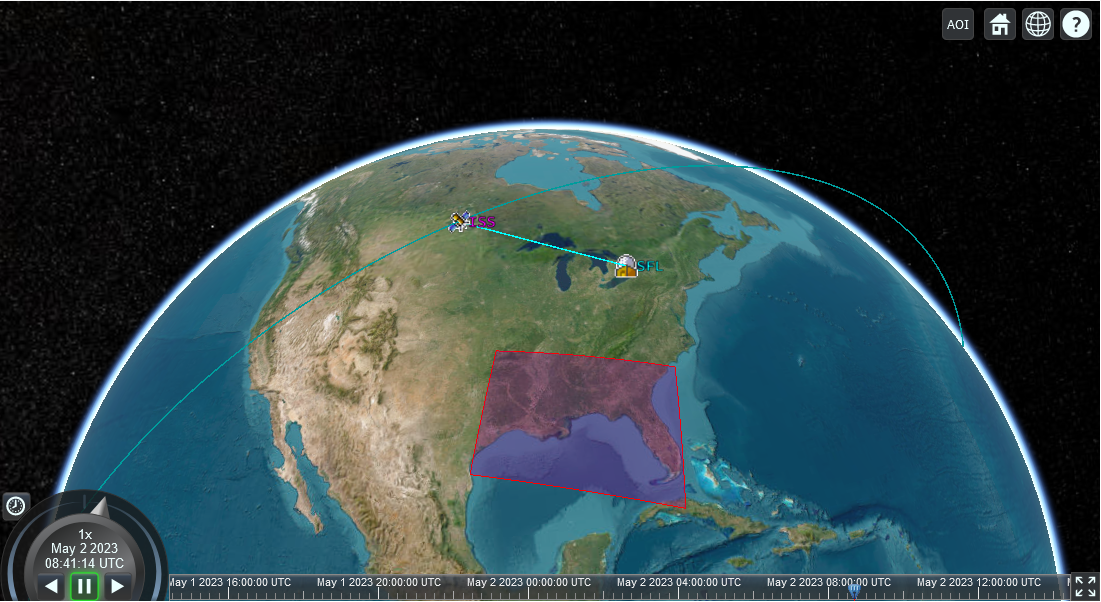
\includegraphics[width=0.7\textwidth]{Cesium_Example_Image.png} 
    \caption{High Level Structure of Mission Model Service}
    \label{fig:mission_model} 
\end{figure}


With a custom-made Cesium handler class, \gls{pops} can visualize:
the Earth, spacecraft, their orbits, ground stations, and can draw polygons on
the Earth.  In addition to displaying information, the handler class also
enables a user to make changes in the viewer which are then reflected in
\gls{pops} itself. The mission model service has many other features including:
database management, opportunity filtering, and scheduling. These features will
be discussed in the WORKFLOW section.  


\subsection{Data Handler}

\subsection{ATU Handler}

\subsection{Opportunity Filter}

\subsection{Scheduler}




\section{Database}

\gls{pops} must be able to retain information, even if it is
shut down or moved somewhere else. It is also necessary that data be stored
such that it does not sit in RAM. For this reason, an SQL database service is
included. It stores all the data necessary for \gls{pops} to function. This
includes but is not limited to satellite information, \gls{tle}s, current and
previous plans, ephemeris data, observation opportunity data, and planned
observations. Using an SQL database allows for effective data storage and
access. There are also no read or write restrictions on an SQL database so data
can be accessed simultaneously by multiple users or services.





\section{Access Time Utilities}


The Access Time Utilities are the fundamental components that enable POPS to be
a planning software. They form the basic building blocks for constraining
observation opportunities. Additional utilities can be added depending on a
mission’s need. The following sections discuss the baseline functionality that
has currently been implemented.


\subsection{Ground Access Utility}

A Ground Access is defined as the time interval during which a satellite can
establish contact with a ground station. A ground station is a point on the
Earth’s surface, identified with geodetic latitude-longitude-altitude
coordinates and an elevation mask. An elevation mask is the angle above the
horizon, at the ground station’s position, at which the satellite can be
considered visible by the ground station. Calculating the ground access for
satellites on a mission is a fundamental task in operations planning. These
time intervals dictate the opportunities for data downlink, command uplink, and
any other communication between the ground segment and satellite. 

The simplest way to compute ground access involves propagating the orbit of a
satellite and checking, at every time step, the position of the satellite
relative to the ground station and testing whether the relative position is
above the elevation mask. While this method is trustworthy and capable of
returning accurate results, its reliance on iterating over an entire satellite
orbit input typically yields a long runtime. This is particularly evident in
the case where a mission has multiple ground stations, multiple satellites, or
a short propagator timestep. The computation time drawback motivates the use of
other algorithms that can determine ground access more efficiently. 

There have been a plethora of papers published on the subject of efficiently
computing ground access over the years. Early work includes Lawton’s
development of a method for calculating ground access for low-eccentricity
satellite orbits by leveraging the Fast Fourier Transform to quickly find a
ground access11. Alfano et al.12 use another technique known as parabolic
blending for constructing the visibility function and finding ground access.
While POPS currently utilizes the simplest method for calculating ground
access, the method that is selected for future implementation is that of Han et
al.13, which uses a self-adaptive interpolation technique to approximate the
waveform of the visibility function. The advantage of this method is its
suitability for all orbit types and orbit propagators, which allows the methods
employed by POPS to generalize for any mission orbit definition. 


\subsection{Swath Utility} 

As discussed in the Terminology section, the concept of an access swath is
defined as a time-series of access regions as a satellite orbits the Earth.
Within \gls{pops}, a swath is represented through a closed curve that describes
the boundary of the cumulative access region of a sensor’s \gls{for} over a
time interval. The process for calculating a swath boundary from an input
ephemeris is described here. 



\subsection{Swath Intersection Utility}

Swath intersection is an important operation for determining what part of a
specified region is observable by a satellite sensor during some time interval.
Regions are polygons on the Earth’s surface whose vertices are oriented
counter-clockwise. The edge between two consecutive vertices is the great
ellipse arc connecting both points. Swaths are also approximated as polygons
provided that the timestep is small enough. The edge between two swath boundary
points being a great ellipse arc is assumed to be a sufficient approximation. 

Polygon clipping techniques are used to find the area of intersection between a
swath and a polygon. First, the swath and polygon vertices are transformed into
2D coordinates. The 2D projection used involves defining a plane that is
tangent to some point on the Earth’s surface. To project a point on the Earth’s
surface to this plane, a vector is drawn from the centre of the Earth towards
the point (its \gls{ecef} coordinates), and the vector is extended towards the
point of intersection of the plane. This type of projection is commonly known
as the Gnonomic projection; its advantage with respect to the polygon clipping
operation is that great ellipse arcs are projected as straight lines. This
means classical 2D polygon clipping techniques can be applied to polygons drawn
on the Earth’s surface. So long as the swath and polygon occupy one hemisphere
of the Earth’s surface, the projection will accurately represent the points of
intersection of the swath and polygon, and any polygon clipping technique can
be applied. 




